%%%%%%%%%%%%%%%%%%%%%%%%%%%%%%%%%%%%%%%%%
% Stylish Article
% LaTeX Template
% Version 2.1 (1/10/15)
%
% This template has been downloaded from:
% http://www.LaTeXTemplates.com
%
% Original author:
% Mathias Legrand (legrand.mathias@gmail.com) 
% With extensive modifications by:
% Vel (vel@latextemplates.com)
%
% License:
% CC BY-NC-SA 3.0 (http://creativecommons.org/licenses/by-nc-sa/3.0/)
%
%%%%%%%%%%%%%%%%%%%%%%%%%%%%%%%%%%%%%%%%%

%----------------------------------------------------------------------------------------
%	PACKAGES AND OTHER DOCUMENT CONFIGURATIONS
%----------------------------------------------------------------------------------------

\documentclass[fleqn,10pt]{SelfArx} % Document font size and equations flushed left

\usepackage[italian]{babel} % Specify a different language here - english by default

\usepackage{lipsum} % Required to insert dummy text. To be removed otherwise

%----------------------------------------------------------------------------------------
%	COLUMNS
%----------------------------------------------------------------------------------------

\setlength{\columnsep}{0.55cm} % Distance between the two columns of text
\setlength{\fboxrule}{0.75pt} % Width of the border around the abstract

%----------------------------------------------------------------------------------------
%	COLORS
%----------------------------------------------------------------------------------------

\definecolor{color1}{RGB}{0,0,90} % Color of the article title and sections
\definecolor{color2}{RGB}{0,20,20} % Color of the boxes behind the abstract and headings

%----------------------------------------------------------------------------------------
%	HYPERLINKS
%----------------------------------------------------------------------------------------

\usepackage{hyperref} % Required for hyperlinks
\hypersetup{hidelinks,colorlinks,breaklinks=true,urlcolor=color2,citecolor=color1,linkcolor=color1,bookmarksopen=false,pdftitle={Title},pdfauthor={Author}}

%----------------------------------------------------------------------------------------
%	ARTICLE INFORMATION
%----------------------------------------------------------------------------------------

\JournalInfo{Progetto del corso \textit{Industry Lab}, Università degli Studi di Milano Bicocca} % Journal information
\Archive{Anno Accademico 2019-20} % Additional notes (e.g. copyright, DOI, review/research article)

\PaperTitle{GP5 - Analisi dei dati e previsione del coefficiente di perdita} % Article title

\Authors{Riccardo Cervero\textsuperscript{1}, Marco Savino\textsuperscript{2}, Luca Lazzati\textsuperscript{3}} % Authors
\affiliation{\textsuperscript{1}\textit{794126, Dipartimento di Informatica, Sistemistica e Comunicazione}} % Author affiliation
\affiliation{\textsuperscript{2}\textit{793516, Dipartimento di Informatica, Sistemistica e Comunicazione}} % Author affiliation
\affiliation{\textsuperscript{3}\textit{?, Dipartimento di Informatica, Sistemistica e Comunicazione}}

\Keywords{Monitoraggio -- Previsione} % Keywords - if you don't want any simply remove all the text between the curly brackets
\newcommand{\keywordname}{Keywords} % Defines the keywords heading name

%----------------------------------------------------------------------------------------
%	ABSTRACT
%----------------------------------------------------------------------------------------

\Abstract{}

%----------------------------------------------------------------------------------------

\begin{document}

\flushbottom % Makes all text pages the same height

\maketitle % Print the title and abstract box

\tableofcontents % Print the contents section

\thispagestyle{empty} % Removes page numbering from the first page

%----------------------------------------------------------------------------------------
%	ARTICLE CONTENTS
%----------------------------------------------------------------------------------------

\section*{Caso di studio} % The \section*{} command stops section numbering

\addcontentsline{toc}{section}{Caso di studio} 

%Spiegazione problema

%------------------------------------------------
\section{Data Preparation}
Il \textit{database} si compone di 296605 osservazioni, descritte da 33 colonne. Tuttavia, è stato necessario focalizzare l'analisi su quelle che presentavano un certo grado di rilevanza e utilità per l'oggetto di studio. Ciò ha comportato la rimozione, durante una prima fase di \textit{pre-processing}, delle variabili che presentavano le seguenti caratteristiche: si manifestavano come un unico valore costante\footnote{Le costanti rimosse sono: \texttt{"Banco"}, \texttt{"Master"}, \texttt{"Picco coppia zero"}, \texttt{"Picco coppia iniziale"}, \texttt{"Media coppia iniziale"}, \texttt{"Velocità 1"}, \texttt{"Picco pressione velocità 2"}, \texttt{"Media pressione velocita 2"}, \texttt{"Picco portata velocità 2"}, \texttt{"Media portata velocità 2"}.}, mostravano una distribuzione eccessivamente sbilanciata verso una sola classe\footnote{È questo il caso di \texttt{"Velocità 2"}, \texttt{"Esito"} e di conseguenza \texttt{"N. Esito"}, \texttt{"Coppia max ciclo"}, \texttt{"Velocità a regime"}.}, erano ridondanti, poco interessanti o erano già state segnalate tali dai fornitori del \textit{dataset}\footnote{Le colonne inutili sono: \texttt{"Codice da Linea"} - identificativo del pezzo -, \texttt{"Media coppia zero"}, \texttt{'Data'} e \texttt{'Ora'}, poiché i dati sono stati raccolti in un arco temporale non uniforme.}. Infine, è stata rimossa una sola riga, poiché penalizzata dalla mancanza dei valori di pressione.
%------------------------------------------------
\section{Analisi preliminari}
Dopo le operazioni di pulizia appena menzionate, si è proceduto ad analizzare in maniera preliminare le colonne rilevanti, per ottenere un primo approfondimento sui descrittori e i rapporti di dipendenza fra gli stessi. 
\subsection{Variabili categoriche}
I dati nominali conservati sono relativi a due precisi aspetti del processo: la segmentazione del lavoro in turni differenti e il programma selezionato per la creazione del pezzo, ovvero la tiplogia di pompa.\\
Per quanto riguarda la prima, è stato necessario aggregare le medesime classi registrate erroneamente in maniera diversa, uniformandone la denominazione. In questo modo, sono state ottenute 5 classi: "A", "B", "C", "D", "0". Le ultime due sono state osservate in minor misura e non specificate inizialmente dai fornitori del \textit{dataset}, e pertanto etichettate come "\textit{non valori}".
\begin{figure}[ht]
    \centering
    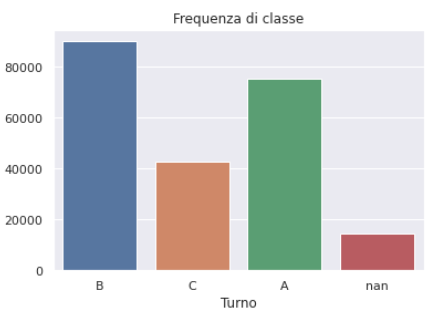
\includegraphics[width=0.9 \linewidth]{turno.png}
    \label{fig:em}
    \caption{\textit{Bar chart} per la visualizzazione delle rispettive frequenze osservate dei turni.}
\end{figure}
Come osservabile in Figura 1, i principali blocchi in cui è organizzato il processo presentano una frequenza diversa: il turno "B" costituisce più del 40\% dei \textit{records}, "A" si presenta nel $\sim$34\% dei casi e "C" nel $\sim$19\%.\\
La composizione del "Programma" mostra un fortissimo sbilanciamento verso la classe GP5 denominata \texttt{18\_GP5\_910\_CW} (Figura 2), che corrisponde alla pompa "\textit{Daimler}". Le restanti tipologie, raggruppate sotto denominazione "Standard", formano in totale meno del 23\% dei casi e sono principalmente rappresentate dalle categorie \texttt{17\_GP5\_430\_CCW} (10.6\%) e \texttt{12\_GP5\_430B\_D1} (8.5\%).
\begin{figure}[ht]
    \centering
    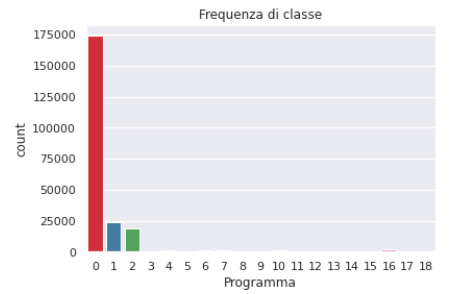
\includegraphics[width=0.9 \linewidth]{prog.png}
    \label{fig:em}
    \caption{\textit{Bar chart} per la visualizzazione delle rispettive frequenze osservate dei programmi.}
\end{figure}
Per una visualizzazione migliore, in Figura 3 è riassunta la distribuzione delle frequenze logaritmiche delle varie classi GP5.
\begin{figure}[ht]
    \centering
    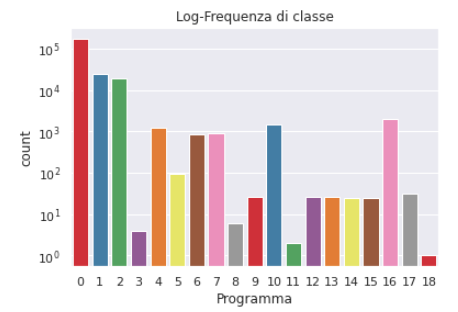
\includegraphics[width=0.9 \linewidth]{proglog.png}
    \label{fig:em}
    \caption{\textit{Bar chart} per la visualizzazione delle rispettive frequenze logaritmiche dei programmi.}
\end{figure}
Tra le variabili categoriche esaminate, "Esito" descrive le eventuali - rarissime - imperfezioni del prodotto. A tal proposito, il 99.5\% delle volte, il risultato è ottimale, mentre l'anomalia più comune è indicata come "scarto picco coppia max fase pulizia iniziale" (0.1\% delle osservazioni).
\subsection{Variabili numeriche}
I dati numerici registrano, per ogni pompa, due principali set di valori, relativi al picco e alla media rispettivamente di pressione (in bar) e portata (in litri all'ora), misurati in corrispondenza di due velocità diverse:
\begin{itemize}
    \item a regime: 2300 \textit{r.p.m}
    \item 140 \textit{r.p.m}
\end{itemize}
Si vedrà che, a prescindere dalla velocità, le due grandezze condividono un'elevatissima dipendenza lineare.
\subsubsection{Descrittori della pressione}
Innanzitutto, le grandezze relative al picco e alla media si distribuiscono in maniera quasi identica nell'ambito della stessa misurazione della velocità (Figura 4). Il range osservato è molto superiore per quanto concerne la velocità a regime. Un riassunto è offerto dalla Tabella 1.
\begin{figure}[ht]
    \centering
    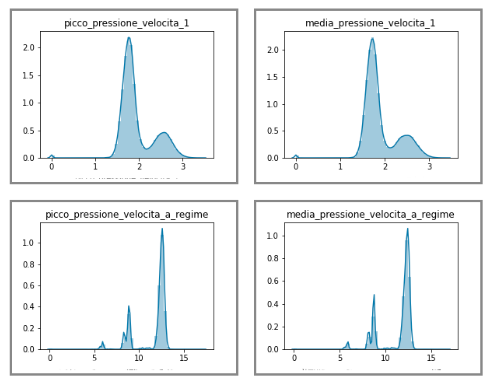
\includegraphics[width=0.9 \linewidth]{press.png}
    \label{fig:em}
    \caption{Distribuzioni delle grandezze relative alla pressione, misurate in corrispondenza della velocità "1" e a regime.}
\end{figure}
{\begin{table}[ht]
\centering
\begin{tabular}[t]{lccc}
\toprule
&Minimo&Media&Massimo\\
\midrule
\textbf{Picco 140rpm}&0.19&1.94&3.45\\
\textbf{Picco 2300rpm}&5.38&11.61&14.21\\
\textbf{Media 140rpm}&0.1&1.88&3.38\\
\textbf{Media 2300rpm}&5.33&11.41&14.01\\
\bottomrule
\end{tabular}
\end{table}}
\subsubsection{Descrittori della portata}
\subsubsection{Altre variabili}
\subsection{Correlazione fra variabili numeriche}
\subsection{Target: coefficiente di perdita}
%------------------------------------------------
\section{Sistema di monitoraggio}
%------------------------------------------------
\section{Limite dinamico di portata}
%----------------------------------------------------------------------------------------
\section{Modelli di previsione}
%----------------------------------------------------------------------------------------
%	REFERENCE LIST
%----------------------------------------------------------------------------------------
\phantomsection
\bibliographystyle{unsrt}
\bibliography{sample}

%----------------------------------------------------------------------------------------

\end{document}
